\documentclass[letterpaper]{article}

\usepackage{aaai}
\usepackage{times}
\usepackage{helvet}
\usepackage{courier}
\usepackage{graphicx}
\usepackage{stfloats}
\usepackage{color}

\usepackage{float}
\floatstyle{boxed} 
\restylefloat{figure}

\usepackage[noend,linesnumbered,algoruled]{algorithm2e}
% %%%%%%%%%%%%%%%%%%%%%%%%%%%%%%%%%%%%%%%%%%%%%%%%%%%%%%
% PDFMARK for TeX and GhostScript
% Uncomment and complete the following for metadata if
% your paper is typeset using TeX and GhostScript (e.g
% if you use .ps or .eps files in your paper):
% \special{! /pdfmark where
% {pop} {userdict /pdfmark /cleartomark load put} ifelse
% [ /Author (John Doe, Jane Doe)
% /Title (Paper Title)
% /Keywords (AAAI, artificial intelligence)
% /DOCINFO pdfmark}
% %%%%%%%%%%%%%%%%%%%%%%%%%%%%%%%%%%%%%%%%%%%%%%%%%%%%%%
% PDFINFO for PDFTeX
% Uncomment and complete the following for metadata if
% your paper is typeset using PDFTeX
% \pdfinfo{
% /Title (Input Your Title Here)
% /Subject (Input The Proceedings Title Here)
% /Author (First Name, Last Name;
% First Name, Last Name;
% First Name, Last Name;)
% }
% %%%%%%%%%%%%%%%%%%%%%%%%%%%%%%%%%%%%%%%%%%%%%%%%%%%%%%
% Uncomment only if you need to use section numbers
% and change the 0 to a 1 or 2
% \setcounter{secnumdepth}{0}
% %%%%%%%%%%%%%%%%%%%%%%%%%%%%%%%%%%%%%%%%%%%%%%%%%%%%%%


\newcommand{\from}[2]{\textcolor{red}{\noindent\textbf{//}\textbf{Note
      from #1:}\textsc{ #2}\textbf{//}}}
      
      \newcommand{\fw}[1]{\texttt{#1}}




\begin{document}
% \title{Transferring Human Spatial Regions from Sensor Data via Analogy}
\title{Representing and Reasoning About Spatial Regions Defined by Context}
% \title{Towards a Cognitive System Than Can Represent and Reason about Spatial Regions Defined by Context}
% \title{Context-Dependent Spatial Regions}
% \title{Qualitative and Analogical Cognition for Spatial Regions Defined by Context}

\author{Matthew Klenk \\ Palo Alto Research Center \\  Palo Alto, CA \\ matthew.klenk@parc.com \And Nick Hawes \\ Intelligent Robotics Lab \\ University of Birmingham, UK \\ n.a.hawes@cs.bham.ac.uk \And Kate Lockwood \\ ITCD Department \\ California State University - Monterey Bay \\ klockwood@csumb.edu  }


 \maketitle
 \begin{abstract}
In order to collaborate with people in the real world, cognitive systems must be able to represent and reason about spatial regions in human environments. Consider the command \emph{``go to the front of the classroom''}. The spatial region mentioned (the front of the classroom) is not perceivable using geometry alone. Instead it is defined by its functional use, implied by nearby objects and their configuration. In this paper, we define such areas as \textit{context-dependent spatial regions} and propose a method for a cognitive system to learn them incrementally by combining qualitative spatial representations, semantic labels, and analogy. Using data from a mobile robot, we generate a relational representation of semantically labeled objects and their configuration. Next, we show how the boundary of a context-dependent spatial region can be defined using \textit{anchor points}. Finally, we demonstrate how an existing computational model of analogy can be used to transfer this region to a new situation. 
 \end{abstract}

 \section{Introduction}

Consider a janitorial robot cleaning a classroom. While performing this task, it encounters a teacher working with a student. The teacher tells the robot to ``start at the front of the classroom'', expecting it to go to the front of the classroom and begin cleaning that area. This response requires that the robot is able to \emph{determine the spatial region in the environment that satisfies this concept}.

The ability to understand and reason about \textit{spatial regions} is essential for cognitive systems performing tasks for humans in everyday environments. Some regions, such as whole rooms and corridors, are defined by clearly perceivable boundaries (e.g. walls and doors). However, many regions to which humans routinely refer are not so easily defined. Consider, for example, the aforementioned region \textit{the front of the classroom}. This region is not easily perceivable using just the geometry of the environment. Instead, it is defined by the objects present in the room (chairs, a desk, a chalkboard), their role in this context (seats for students to watch a teacher who writes on the chalkboard) and their configuration in space (the seats point toward the chalkboard). In this paper, we will refer to such regions as \textit{context-dependent spatial regions}. 

% Pat:
% Finally, let me urge you to include specific claims in your paper and
% to provide evidence that supports them. Such evidence can take many
% forms, from experimental studies to proofs to compelling arguments,
% but making this explicit will improve your chances.


Representing and reasoning about context-dependent spatial regions is beyond the capabilities of current cognitive systems, yet it is an important ability for three reasons:
\begin{itemize}

\item{If cognitive systems are to collaborate with humans in everyday environments, then they must be able to represent and reason about the spatial regions humans refer to. Many regions are best defined in a context-dependent manner, for example, a kitchen in a studio apartment, an aisle in a church or store, behind enemy lines in a military engagement, etc.}


\item{Cognitive systems must integrate different types of information, including geometric, semantic, and functional knowledge. The identification of context-dependent spatial regions provides a suitable task for studying this integration. Only through such integration could a system determine, for example, whether a banquet hall has a dancefloor depending on the arrangement of the room.}

\item{Cognitive systems must adapt their knowledge and experience to new situations. While humans do not demonstrate mastery after seeing a single example of a new concept, they are able to begin using it immediately, whilst incrementally refining it over time (cf. one-shot learning~\cite{Fei-Fei/etal:2006}). This has important implications with respect to the amount of knowledge engineering and training time required to create a cognitive system. For example, having trained a mobile robot to understand the front of one classroom, it is desirable for it to be able to identify the front of other classrooms and similar areas (e.g. theaters) without additional tutoring.}
\end{itemize}

\begin{figure*}[t!]
  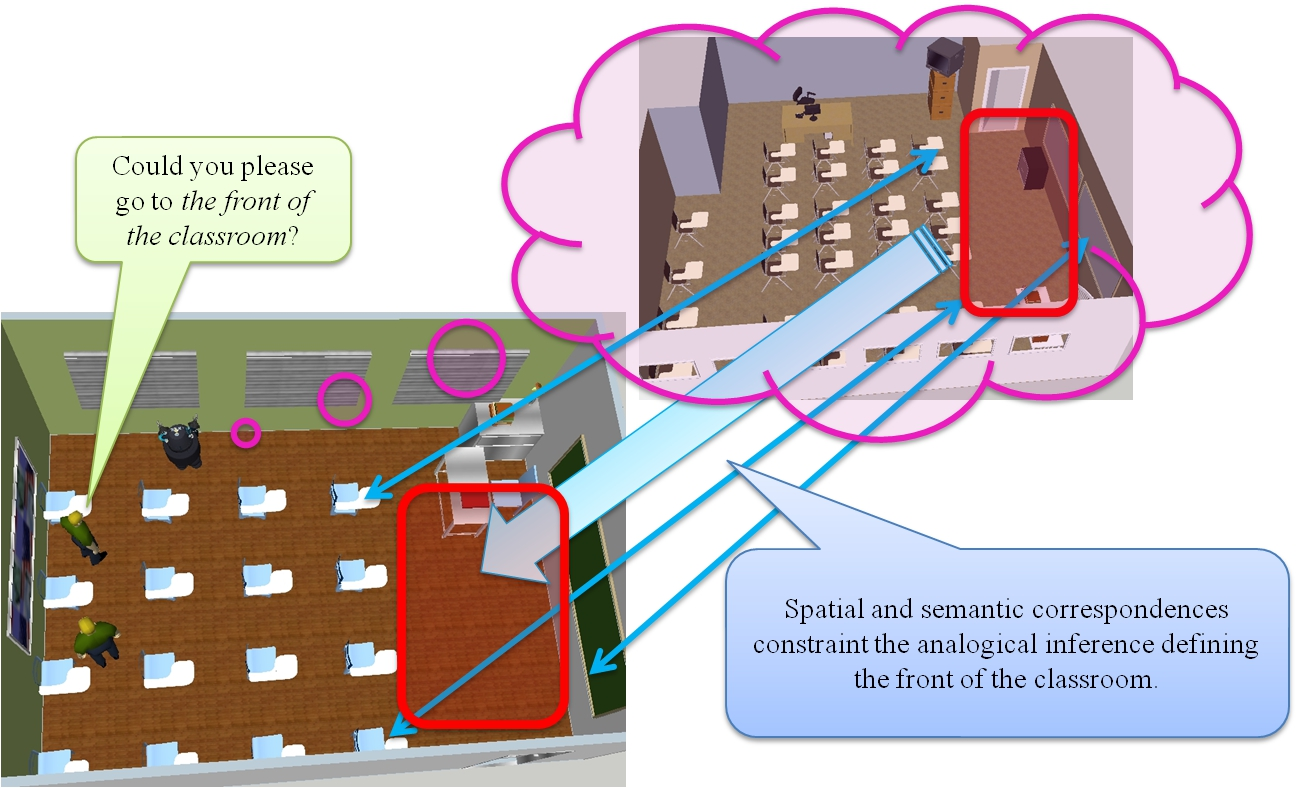
\includegraphics[width=\textwidth]{example1.jpg}
  \caption{
This image demonstrates the behavior we desire of our cognitive system. The robot is able to identify the front of the classroom by analogy to a previously labelled example. To do this it must identify the correspondences between the example and its current environment (the desks in the front row and chalkboards) and then transfer the spatial region (the front of the room is between these entities).}
  \label{fig:example}
\end{figure*}

Figure \ref{fig:example} illustrates our approach for understanding context-dependent spatial regions via analogy. Our first assumption is that these regions can be defined using qualitative spatial representations~\cite{Cohn:2001}. Our second assumption is that geometrically and semantically similar areas will feature similar context-dependent spatial regions, and that these can be transferred through analogy. 

In the context of the symposium on ``Advances in Cognitive Systems'' we are making two specific claims:

\begin{enumerate}
\item Understanding context-dependent spatial regions is an essential ability for a cognitive system that must interact with humans.
\item This ability can be realized in an artificial cognitive system through the combination of a sensor-based spatial model, qualitative spatial representations, and analogy.  
\end{enumerate}

\noindent We appeal to the reader's experience and intuition to evidence the first claim. To support this, we have already provided a number of examples of situations in which humans rely on context-dependent spatial regions, but we have not done any systematic collection or analysis of real-world situations in which they occur. To evidence the second claim, we present the results of developing an extension to an existing cognitive system that enables it to learn context-dependent spatial regions by example. 

The rest of the paper is structured as follows. First, we describe how we generate qualitative spatial representations from the spatial model of an existing system. Second, we describe how we define context-dependent spatial regions using \textit{anchor points} \cite{Klenk/etal2005}, i.e., symbolic descriptions that tie conceptual entities to geometric points. Next, we use the structure-mapping model of analogy \cite{Gentner1983a} to transfer knowledge from an existing context-dependent spatial region to a new situation. Finally, we discuss some limitations of our current implementation, and position it with respect to previous work and cognitive systems in general.

\section{From Sensors to Semantics}

Our approach to representing and reasoning about context-dependent spatial regions requires the existence of qualitative spatial representations~\cite{Cohn:2001} describing the relationships between the entities a cognitive system perceives (including objects, groups, and regions). By adding semantic labels, or types, to each entity, we are able to reason about the geometric \emph{and} conceptual characteristics of the system's environment. The following sections describe how we generate appropriate qualitative spatial representations using the spatial model of an existing, state-of-the-art, cognitive system.

\subsection{The Dora System}

\begin{figure}[t!]
  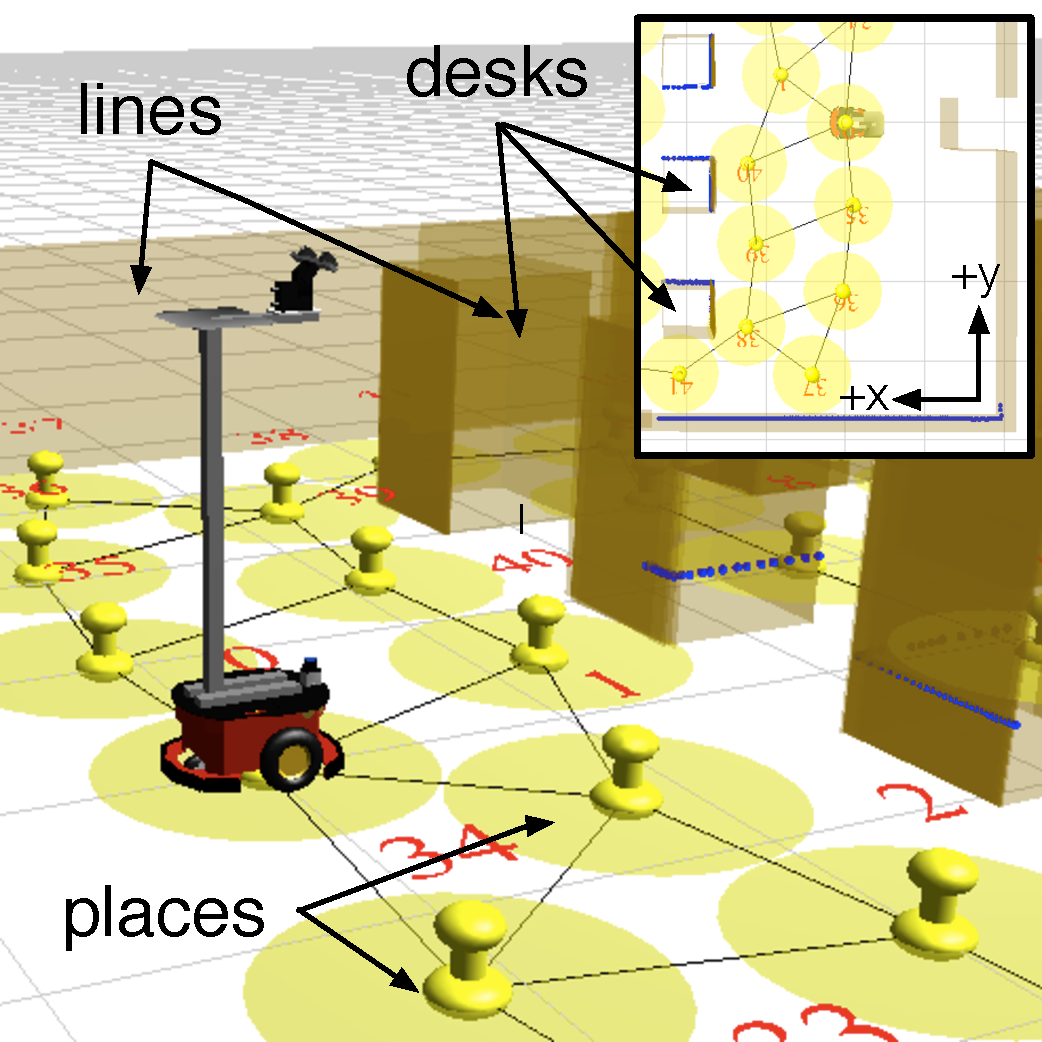
\includegraphics[width=\columnwidth]{images/classroom-peekabot-annotated.pdf}
  \caption{A visualization of Dora's existing spatial model taken from the running system. Walls are visualized where flat surfaces (walls, desks and other objects) are detected during SLAM.}
  \label{fig:dora-spatial}
\end{figure}

We base our work on Dora, a mobile cognitive robot with a pre-existing multi-layered spatial representation~\cite{Hawes/etal:2011}. In this paper, we focus on the basic elements of this spatial model. For more information on Dora's other competences, see recent papers, e.g.~\cite{Hawes/etal:2011,Hanheide/etal:2011}.

In the simplest terms, Dora's spatial model can be treated as two layers: a \emph{metric layer} and a \emph{place layer}. A visualization of these from the running system is shown in Figure~\ref{fig:dora-spatial}.
% Metric layer
The metric layer is a collection of lines in a 2D global coordinate frame. These lines are generated by a  process which uses input from the robot's odometry and laser scanner to perform simultaneous localization and mapping (SLAM). Lines in this SLAM map represent features extracted from laser scans wherever a straight line is present for long enough to be considered permanent. In practice, lines are generated at the positions of walls and any other objects that are flat at the height of the laser (e.g. foot stools, bins, closed doors etc.). The robot's location in the metric layer is represented as a 2D position plus an orientation.
% Place layer
As the robot moves around in the world, the free space it passes through is discretized into a graph of connected nodes $1m$ apart. We refer to these nodes as \emph{places} and the graph of connected places forms the spatial model's place layer. The robot's location in the place layer is represented by a pointer to a place. Places allow Dora to reason about space in basic qualitative ways, e.g. by clustering places into rooms based on the presence of doorways, and provide a representation of space capable of facilitating behavior planning.
% Objects
Dora is capable of using vision to recognize predefined objects. Recognition can either be triggered through autonomous visual search or a a user's command. When an object is detected it is represented in the place layer relative to Dora's current position. The recognizer associates each object with a label that was provided during a training phase. In our current work, these labels are used directly in analogical processing. We use a convex hull around the places in a room to represent its area, and the 2D locations of perceived objects to create the qualitative spatial representations in the next section.

% simulation
As the purpose of this paper is to explore the possibility of using qualitative spatial reasoning and analogy on top of Dora's spatial model, we decided to perform our research using the Player/Stage hardware abstraction layer and simulation tools~\cite{GerkeyVaughanHoward03} rather than on a real robot. This allows us to run the Dora system \emph{mostly unchanged} in a controlled simulation environment, rather than deal with some of the unrelated challenges of running the robot in the real world. The key difference is that the sensor readings are free of noise in the simulated world. This is particularly significant where vision is concerned, as Dora's object recognizer is replaced entirely by a simulated blob detector which is always correct. Beyond this, the functionality of the system remains unchanged, and, crucially, the representations our work builds on will be the same when the system is run in the real world.  


\subsection{Qualitative Spatial Representation Extraction}

Given data from Dora's spatial model, we compute the following qualitative spatial representations. First, we extract the object and room entities from the sensor data. Next, we determine the qualitative spatial relationships between these entities. For the room, we compute its region as a convex hull around the set of points. For the objects, we consider only their centroids. For each pair of adjacent objects, we compute topological and positional relationships. Adjacency is determined by creating a voronoi diagram as is standard geometric reasoning \cite{Forbus/etal2003}. For the topological relationships, we use the region connection calculus, RCC8, \cite{Cohn:2001}. For positional relations, we use two predicates \fw{leftOf} and \fw{below}. An entity is \fw{leftOf} another if the x coordinate of its centroid is less than that of the other entity's. An entity is \fw{below} another if the y coordinate of its centroid is less than that of the other entity's. Objects whose x or y coordinates are within a threshold of one another will not be related by \fw{leftOf} or \fw{below} positional relations.

%\from{Nick}{I have changed the below paragraph to match the actual numbers and images. I've marked what I changed}
%Desk 1 and Desk 2 are not labeled in the Figure.

Consider the situation in Figure~\ref{fig:dora-spatial} where the robot is facing two desks in a row\footnote{Please note that although the desks in front of the robot in Figure~\ref{fig:dora-spatial} appear distributed left to right from the robot's current position, they are actually distributed bottom to top, according to our definitions, in the global coordinate frame.}. Because we represent the desks as distinct points, \fw{(rcc8-DC Desk1 Desk2)} states that they are disjoint. To account for their relative positions, neither \fw{(leftOf Desk1 Desk2)} nor \fw{(leftOf Desk2 Desk1)} are true because the x coordinate of \fw{Desk1} is within a threshold of the x coordinate of \fw{Desk2}. The statement \fw{(below Desk1 Desk2)} is true because \fw{Desk1} has a lower y coordinate. Each desk is also related to the room by the non-tangential proper part relation, \fw{rcc8-NTPP}. These qualitative spatial relationships provide the structure necessary for analogical processing.

\subsection{Representing Context-Dependent Spatial Regions}

To enable analogical transfer, it is necessary to represent context-dependent spatial regions symbolically. We do this using \textit{anchor points} \cite{Klenk/etal2005} which are symbolic descriptions linking a conceptual entity to a particular point on a perceived entity.  A context-dependent spatial region is a conceptual entity, and the objects in the room and the room itself are perceived entities. As stated previously, the room is represented by a set of points. Anchor points are created using unary functions over a percieved entity. For example, \fw{(CentroidFn Area1)} represents the centroid of geometric extent of \fw{Area1}. We use anchor points to specify the boundary of the context-dependent spatial region using the \fw{regionBoundary} relation. For a particular classroom, we are able to define the front of the room as the region bounded by the leftmost top point of the room, the whiteboard, the leftmost bottom point of the room, and each of the desks in the front row. After we have defined the boundary of the region, we assign it a semantic label using the \fw{regionType} relation. Therefore, each context-dependent spatial region has one type and a variable number of boundary points.
%\from{Nick}{This is crying out for a diagram, perhaps on the stage map of classroom 1.}
%\from{Nick}{You mention chalkboard above, but it is not anywhere else in the below example.}
%\from{Klenk}{We will do for Figure 5.}

\begin{figure}[h]
	{\fontsize{8}{8} %%Because aaai.sty overrides usual font size commands
  
\fw{(regionType CDSR1 FrontRegion)\\
(regionBoundary CDSR1 (LeftmostTopFn Room1))\\
(regionBoundary CDSR1 (LeftmostBottomFn Room1))\\
(regionBoundary CDSR1 Desk1)\\
(regionBoundary CDSR1 Desk2)\\
(regionBoundary CDSR1 Desk3)\\
(regionBoundary CDSR1 Desk4)\\
(regionBoundary CDSR1 Whiteboard0)\\
}}
  \caption{Representing the front of the classroom context-dependent region \fw{CDSR1}}
  \label{fig:cdsr-reps}
\end{figure}

Figure \ref{fig:cdsr-reps} contains the symbolic description for the front of classroom \fw{Room1} which is pictured in the top left of Figure~\ref{fig:dora-maps}. The anchor points (connected in green in Figure~\ref{fig:dora-maps}) define the region. \fw{(LeftmostBottomFn Room1)} and \fw{(LeftmostTopFn Room1)} are the points with the lowest x coordinate out of the set of points defined as the top and bottom of \fw{Room1} respectively. The sets of points representing the top and bottom of the classroom are found by selecting the points defining the area within a threshold of the area's maximum or minimum y coordinate. The other corners of the context-dependent spatial region are defined by the four desks and the whiteboard. Because perceived objects (e.g. the desks) are defined as single points, they can serve as anchor points directly. The semantic label \fw{FrontRegion} ties the geometric extent of the boundary points to a conceptual region. This definition for the front of the classroom is specific to \fw{Room1} and its entities. It is clearly context-dependent because its extent is dependent on the arrangement of the anchor points used to define its boundary. If the desks were in a different position then the region would cover a different extent (e.g. if they were closer to the whiteboard then the region would be smaller). 


% In the next section, we describe how to transfer these environment-specific representations to new situations via analogy.

\section{Analogical Transfer of Spatial Regions}

% While this work focuses on how analogy enables inferences from specific examples to new situations, but its role in the larger cognitive system this work envisions cannot be ignored. 

We assume that a cognitive system will have a way of initially acquiring examples of context-dependent spatial regions, e.g., by being taught by a human through dialogue, sketching, or hand-coding. As stated previously, to avoid burdening potential tutors with the task of teaching the system every context-dependent spatial region individually, it is desirable for a cognitive system to be able to automatically recognize similar regions after its initial training. For example, after training a janitorial robot in just one classroom, it should be able to identify similar regions in the other classrooms in the building. Motivated by the learning and generalization abilities of humans, we have chosen analogy to tackle this problem.

Analogy is an essential cognitive process. In humans, analogical processing has been observed in language comprehension, problem-solving, and generalization \cite{Gentner2003}. The structure-mapping theory of analogy and similarity postulates this process as an alignment between two structured representations, a \textit{base} and a \textit{target} \cite{Gentner1983a}. This alignment process is governed by three constraints: \textit{identicality}, \textit{parallel connectivity}, and \textit{one-to-one mapping}. The identicality constraint provides a strong preference for only allowing identical predicates to match. Parallel connectivity states that if two predicates are matched then their arguments must also match. The one-to-one mapping constraint requires that each element in the base corresponds to at most one element in the target and vice versa. To select between competing mappings, the \textit{systematicity} principle prefers mappings that are highly interconnected and contain deep chains of higher order relations over mappings with an equal number of relations which are independent from each other.

The Structure-Mapping Engine (SME) \cite{Falkenhainer1989a} performs analogical matching. Given two structured representations as input (the base and target), SME produces one or more mappings. Each mapping is represented by a set of \textit{correspondences} between entities and expressions in the base and target.  Mappings also include \textit{candidate inferences} which are conjectures about the target using expressions from the base which, while unmapped in their entirety, have subcomponents that participate in the mapping's correspondences. SME operates in polynomial time, using a greedy algorithm \cite{Forbus/etal1994}.

\begin{figure}[h]
  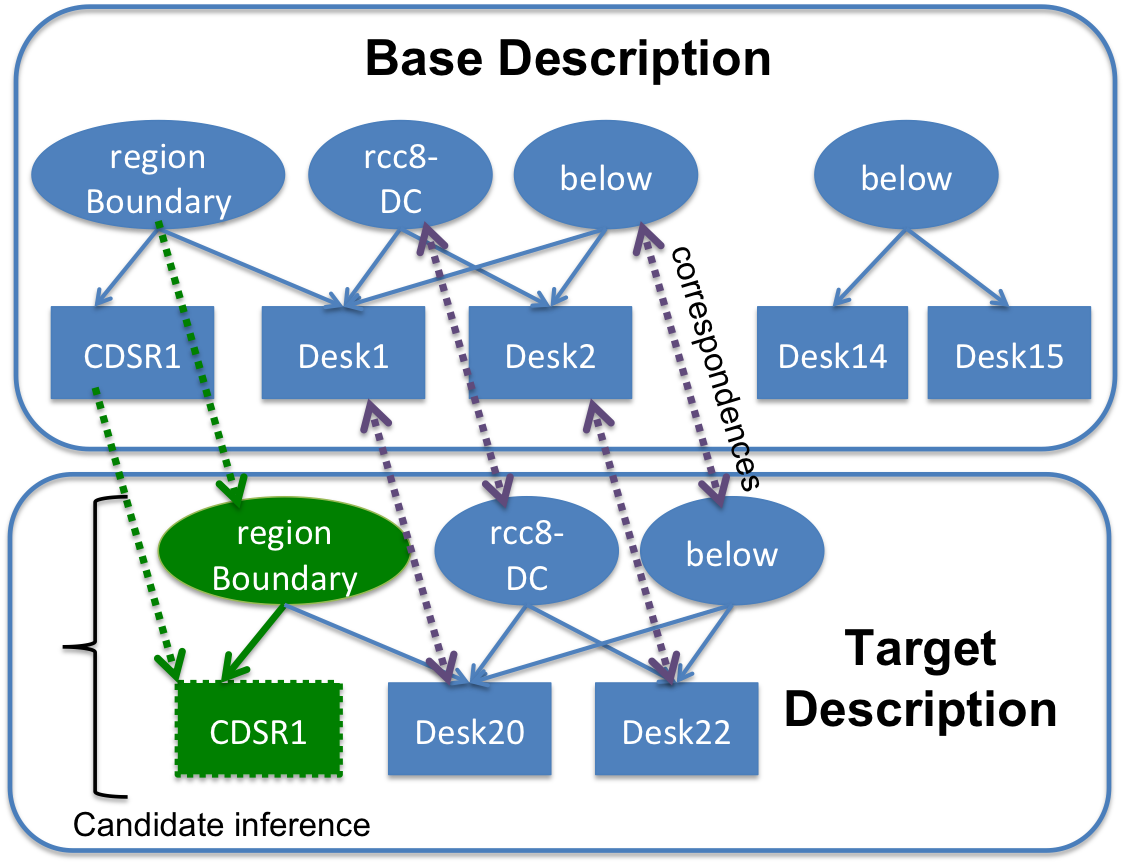
\includegraphics[width=\columnwidth]{analogy2.png}
  \caption{Analogical mapping between four base expressions and two target expressions. Ovals and squares represent relations and entities respectively. Purple dashed bi-directional arrows are the correspondences between the base and target, and the green dashed arrow, oval, and square represent a candidate inference projected into the target.}
  \label{fig:analogy}
\end{figure}

Figure \ref{fig:analogy} illustrates a sample mapping between four base expressions and two target ones. Each oval represents a binary predicate, and its two entity arguments are represented by squares. SME generates a mapping between the base expressions \fw{(rcc8-DC Desk1 Desk2)} and \fw{(below Desk1 Desk2)}, and the  target expressions \fw{(rcc8-DC Desk20 Desk22)} and \fw{(below Desk20 Desk22)}. This is done in the following manner. First, the predicates of these expressions are placed in correspondence by the identicality constraint. Next, parallel connectivity aligns their arguments, \fw{Desk1} with \fw{Desk20} and \fw{Desk2} with \fw{Desk22}. While there is another \fw{below} statement in the base about two desks, it cannot correspond to either of the target expressions in the same mapping due to the one-to-one constraint. In Figure \ref{fig:analogy}, these correspondences are highlighted by the purple hashed bi-directional arrows. Next, SME creates a candidate inference for the expression \fw{(regionBoundary CSDR1 Desk1)}, because \fw{Desk1} participates in the mapping. The candidate inference is stated as \fw{(regionBoundary (:skolem CSDR1) Desk20)}. \fw{:skolem} is used to denote entities that do not exist in the target description but are included in the candidate inferences. In this case, the candidate inference states that there is something like \fw{CSDR1} in the target, and its boundary includes \fw{Desk20}. Note that inference is selective, with no candidate inferences generated for the entirely unmapped \fw{below} expression. Next, we describe how we use the results of an analogy to infer a context-dependent spatial region in the target.
 
% It feels odd having this as a separate subsection
%\subsection{Initial Approach}\label{sec:approach}

In our system, the base and target representations consist of the identified objects from Dora's spatial model drawn from two different runs in two different environment, plus the qualitative spatial relationships computed on top of these. The base also contains a labeled context-dependent spatial region that is sought in target environment. We use SME to create an analogical mapping between the base and target. The result of this mapping is a set of correspondences and a set of candidate inferences. We transfer context-dependent spatial regions as follows. First, we identify the context-dependent spatial region entity of the sought semantic type in the base. This entity should not participate in the mapping, but should be included as \fw{:skolem} expressions in the candidate inferences. To transfer this entity to the target, we collect the candidate inferences resulting from the \fw{regionBoundary} statements in the base that mention the base entity. The second arguments of these candidate inferences are anchor points in the target environment. Therefore, to identify the context-dependent spatial region in the target, we create a new entity, assign it the semantic type of the sought region, and define its boundary using the anchor points from the candidate inferences.

\section{Example}

\begin{figure}[t]
  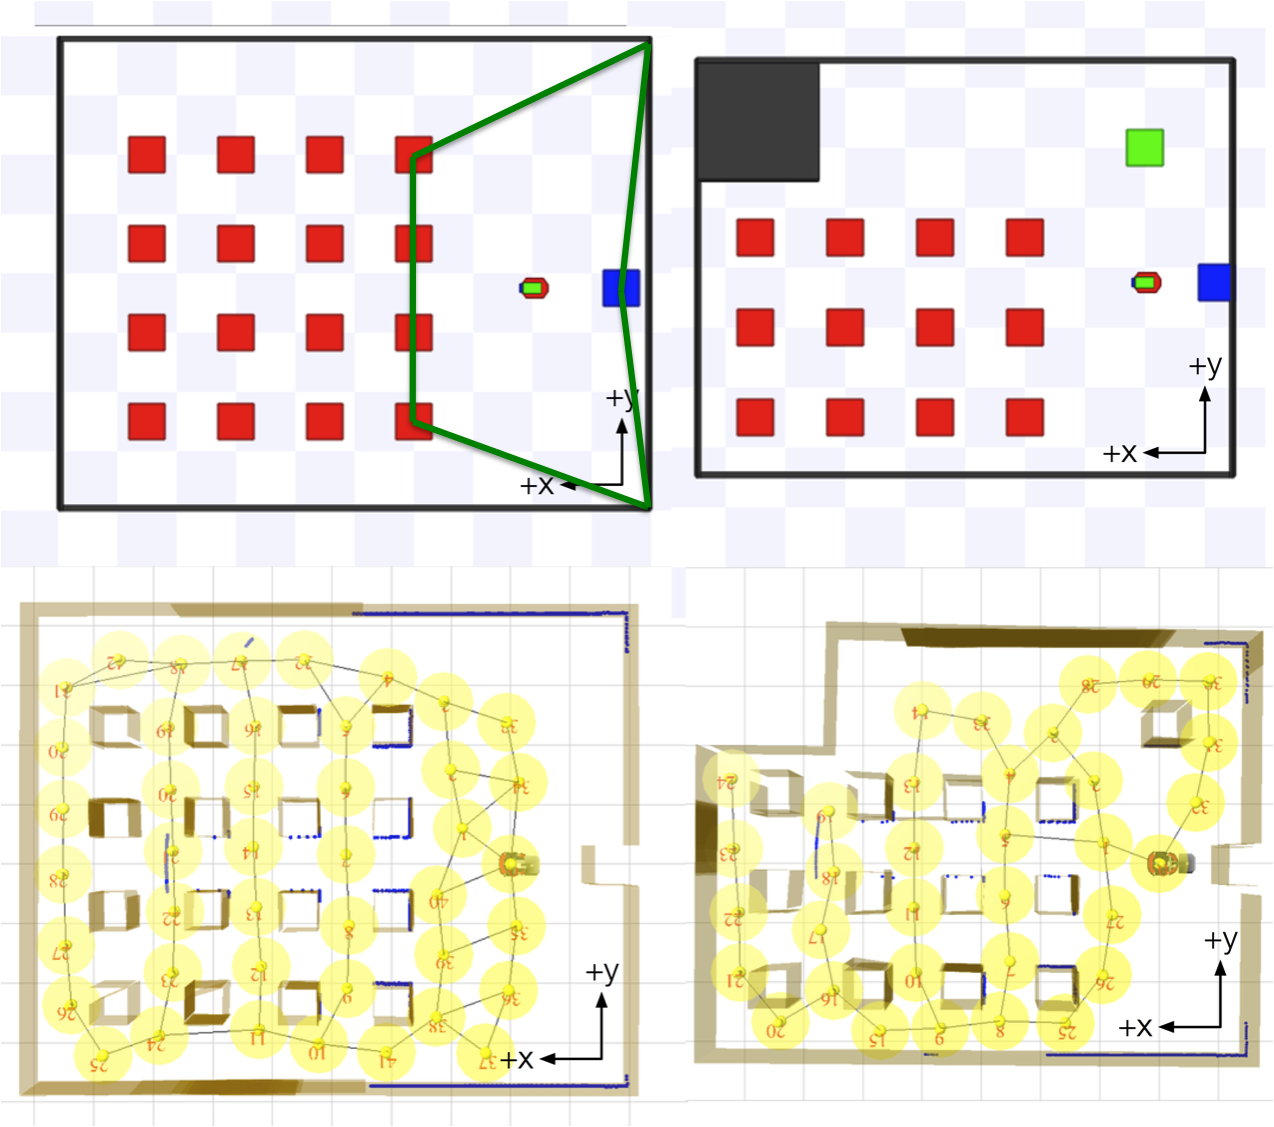
\includegraphics[width=\columnwidth]{images/classroom-maps-axes-annotation.png}
  \caption{The top two images show the Player/Stage classroom simulations used in the example, with the base on the left and the target on the right. The desks are simulated as red boxes, and the chalkboard and lectern (where present) as blue and green boxes respectively. Furthermore, the solid green line in the base connects the boundary points of the front of the room. The lower two images show the metric and place maps generated by Dora during the example runs.}
  \label{fig:dora-maps}
\end{figure}

Using the previously described techniques, we have implemented a system capable of performing an inference similar to the one presented in Figure \ref{fig:example}. The base and target cases are created by running the Dora system on the two different simulated classroom worlds shown in Figure~\ref{fig:dora-maps}. In each case, Dora is manually driven around the room to allow it to create metric and place maps. Once the map is created, Dora is then driven in front of each object and the visual recognition system is run, resulting in the objects being added to the place layer. 

The data from Dora's spatial model is then passed on to the qualitative spatial representation generator. In the base case, there are 16 desks and a chalkboard. There are two other entities in the case: the room area and the context-specific spatial region representing the front of the room. The case includes a total of 96 expressions relating the 19 entities. Nine of these expressions are used to define the boundary of a context-specific spatial region representing the front of the room: the four desks in the front row, the chalkboard, and the leftmost bottom and leftmost top of the room. The target case includes only 12 desks arranged in three columns of four, a chalkboard and a lectern. The target case includes 73 statements and 14 entities.

SME generates an analogy between the base and target cases enabling the transfer of the symbolic description of the front of the room to the new situation. The resulting analogy includes 62 correspondences between the entities and expressions in the base and target and 53 candidate inferences.  All seven \fw{regionBoundary} statements in the base appear as candidate inferences. Five of the anchor points are exactly correct, the leftmost corners of the room, the chalkboard and two of the desks in the front row. The other two analogically transferred anchor points are to the lectern and a desk in the third row. Figure \ref{fig:success} illustrates the region created by the seven boundary points in the target environment. While this region is not identical to how a human would specify it, our system is able to produce a fairly accurate context-dependent spatial region in a new environment from a single example.

\begin{figure}[h]
  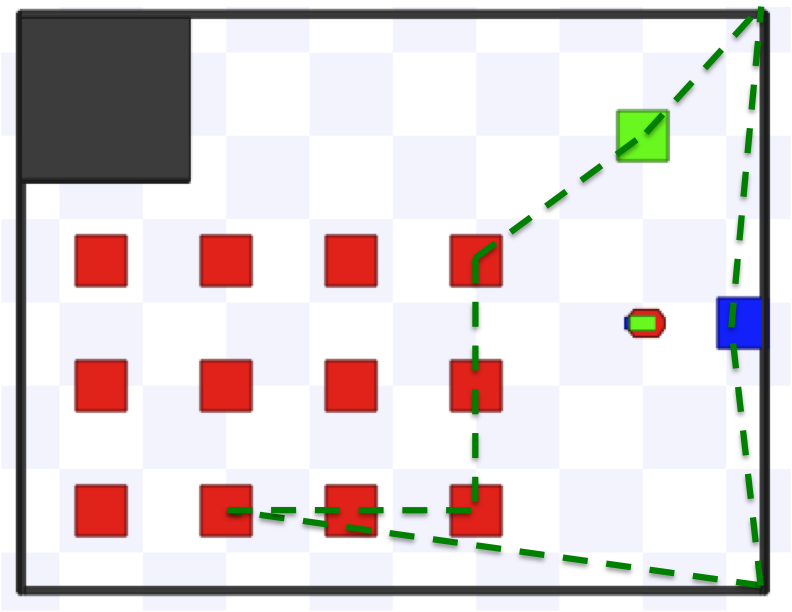
\includegraphics[width=\columnwidth]{images/target-success.png}
  \caption{Successful analogical transfer results in the identification of the front of the room as the green dashed trapezoidal region. The red boxes in rows are the identified desks, the blue box along the wall is the chalkboard, the green box is the lectern, and the green and red object is Dora.}
  \label{fig:success}
\end{figure}

\section{Limitations of Initial Approach}

The spatial transfer algorithm described in here has a number of limitations to be addressed in future work.  First, we have not incorporated a memory retrieval mechanism, such as MAC/FAC \cite{forbus/etal1995}.  As a cognitive system gains experience in different environments, it will have access to a range of context-dependent spatial regions defined in a variety of task situations. To retrieve an analogous example, the agent must select the most similar environment that contains a labeled example of the sought after region type. This extension is fairly straightforward, but beyond the scope of this paper. Second, our initial approach ignores a number of potentially relevant pieces of information. After the context-dependent spatial region has been identified in the target environment, its qualitative spatial relationships could be compared with those from the base to either refine the region or provide a confidence measure for the inference. In our example, the transferred region contains the bottom desk in the second row, but the corresponding region does not contain any desks topologically. Third, our algorithm uses an absolute reference frame. Therefore, the environments must be oriented in a similar fashion to successfully transfer a context-dependent spatial region. We can overcome this limitation by performing a series of analogies between the base and the target in which we rotate the base and select the analogy with the best mapping. Finally, more advanced qualitative spatial relationships should improve performance. For example, recognizing all the desks as one region, or grouping them into rows or columns, would provide a better level of abstraction for this task.

\section{Related Work}

Typical approaches to spatial representation for mobile robots tend to focus on localization, and thus mostly represent the world uniformly without subdivision into meaningful (semantic) units \cite{Thrun02a}. When a more structured representation is required (e.g., for behavior planning or human-robot interaction), topological maps (i.e., graphs of connected regions) are usually built on top of these metric representations using various landmark-detection techniques to segment regions, e.g. door detection \cite{Hawes/etal:2009b} or clustering of perceptual features \cite{Peltason/etal:2009a}. While capable of recognizing regions, these approaches do not consider the semantic information necessary for identifying context-dependent spatial regions. While steps have been taken toward incorporating this knowledge  (i.e. the types of objects present and their arrangement) into spatial representations, current approaches fall short of representing the types of regions discussed in this work. For example, a number of systems attempt to recognize the category of a room by the objects present within it \cite{Hawes/etal:2010b}, and others are able to mediate their behavior when certain functional contexts are detected (e.g. the areas near doors \cite{Zender2008a}).

% Nick: Goal reasoning is a separate issue entirely, and one for a different paper
 % Additionally, existing systems which are able to reason about their behavior are not able to do so with reference to the spatial extent of their goals, and thus would also fail to generate the desired behavior on this count. 

There is mounting evidence that analogy, operating over structured qualitative representations can be used to simulate a number of spatial reasoning tasks. Forbus \textit{et al.} showed that analogy between course of action diagrams could be used to identify potential ambush locations in new situations by focusing on only the relevant aspects of sketched battle plans \cite{Forbus/etal2003}. A core contribution of their work was the definition of a \textit{shared similarity constraint} between a spatial reasoning system and its user; where users and spatial reasoning systems agree on the similarities between situations. This has close parallels to what we are trying to accomplish, where a cognitive system is able to reason about context-dependent spatial regions by identifying the same salient features as its human user. The anchor points in our work were originally used in teaching a system how to solve problems from the Bennett Mechanical Comprehension Test that require spatial and conceptual reasoning. For example, identifying which wheelbarrow will be more difficult to lift based on the relative locations of its loads as depicted in a sketch \cite{Klenk/etal2005}. In that work, the anchor points defined the endpoints of lines. We go beyond that result to use anchor points to specify 2D regions.  The combination of analogy and qualitative representation has been shown to be flexible enough to model problems at different levels of refinement (e.g. edges, shapes, groups) \cite{Lovett&Forbus2011} and to combine semantic as well as geometric information in spatial reasoning tasks (e.g. \cite{Lockwood/etal2008}). Our work demonstrates that the combination of analogy and qualitative spatial representations is useful for problems in cognitive mobile robotics. 
% Therefore, we hope and expect to see more research combining these three fields.

\section{Discussion}

% Nick: All this reptetition and probably unnecessary
% Klenk: I like the repetition. I think it is really important to drive home the cognitive systems story here.

Our first claim for this work is that in order for artificial cognitive systems to collaborate with human users, they must be able to understand and reason about the types of spatial regions that humans use. In particular we have identified context-dependent spatial regions, i.e., regions defined by their geometric, functional, and semantic relations to surrounding entities, as an important type of region that cannot be represented by current systems. Addressing this problem is important as such regions are ubiquitous in human environments and communication, ranging from regions in everyday experience (e.g. aisles, marketplaces) to domain-specific regions (e.g. the ``pocket'' in American Football). 

In addition to addressing a specific need in human-robot interaction, developing a cognitive system able to represent and reason about context-dependent spatial regions is important for two further reasons. First, as these regions are not defined solely by their geometry, we must investigate approaches that integrate different types of knowledge. This is a key problem in cognitive systems work in general. Second, in order to reduce the burden on developers and users, a cognitive system that understands one type of context-dependent spatial region should be able to use this understanding to recognize similar regions in other areas. Developing such a generalization ability (particularly one that can work incrementally from a small number of examples) is another general challenge for the cognitive systems community.

Our second claim in this work is that the combination of a sensor-based spatial model, qualitative spatial representations, and analogy provides a potential solution to the aforementioned problems. We presented results from an initial proof-of-concept implementation that supports this claim. This system is able to transfer, via analogy, context-dependent spatial regions defined using anchor points over logical representations consisting of  object types and qualitative spatial relationships inferred from sensor data. Whilst the system has a number of limitations, and the transferred context-dependent spatial region presented does not perfectly match human expectations, it validates further development of our approach. 

To support the definition of new spatial regions which the robot should be aware of, it is desirable to integrate a sketching interface on top of a visualization of the spatial knowledge the robot already has. Sketching \cite{Forbus/etal:2009a} is often used by humans to convey new ideas and concepts, making this a natural interface for human-robot interaction. When faced with an unknown context-dependent spatial region, the mobile robot could then ask a human to define the region using \textit{sketch annotations} over its representation \cite{Klenk/etal2005}. 

For mobile robots, spatial understanding is required to enable the pursuit of spatially-defined goals (e.g the goal that the front of the classroom is clean). Consequently, spatial understanding should be evaluated with respect to a cognitive system's actions in its environment. The minimal performance for spatial understanding is that the cognitive system is able to navigate to context-dependent spatial regions. A longer term research project involves reasoning about potentially conflicting goals with overlapping spatial extents. A cognitive system should be able to combine them to generate new goals to pursue. The scenario in Figure \ref{fig:example} exemplifies this process of combining goals through spatial extent, when the robot generates the goal of cleaning the front of the classroom. With the proliferation of mobile robots, sensors and computation, new ideas, such as, context-dependent spatial regions, have the potential to reshape how users interact with cognitive systems.

\section{Acknowledgments}

The authors would like to thank Jeffery Usher for providing the code to compute Voronoi diagrams. The research leading to these results has received funding from the European Community's Seventh Framework Programme [FP7/2007-2013] under grant agreement No. 215181, CogX.

\bibliography{understanding-human-spatial-regions} \bibliographystyle{aaai} \end{document}
